\section{Data Mining}
\label{sec:dm}

For this project, to reiterate, we are attempting to predict job salaries given some meta information in both categorical and free text forms
about the job. The training set provided by Kaggle to issue this challenge is as astounding 244,000 training instances. This being the case,
Weka was not an appropriate solution to use as a data mining tool as holding this large amount of data in main memory while preforming standard
data mining operations such as SVM on it would have been devastating in time and space. Another issue with this size of data are run times, especially when 
multiple attempts and different data manipulations will need to be preformed. With these issues present, it is important to either write
our own algorithms for speed and size, or use a pre-existing tool to handle these scenarios for us. We went with the latter option.\\

Solving these issues, we found the data mining tool known as Vowpal Wabbit (VW). VW is a command line based data mining tool originally
created by Yahoo! Research but was later and more recently sponsored by Microsoft Research. VW was designed to be a fast and lightweight
tool from the beginning and accepting of extremely large data sets. VW has a large array of available data mining algorithms, however,
its most prominent algorithm (and algorithm used for this project) is know as the sparse gradient descent (GD) on a loss function.\\

The gradient descent algorithm is a similar structure to the type of gradient descent used in the logistic regression which was taught
in the SENG474 data mining class. The main difference here is the use of the weight vector in VW's gradient descent. The weight vector
that VW uses has $2^b$ weights (where b is the specified by the b option on the command line). What this really means is that each feature
as show in the data preparation section of the VW input, gets hashed to a particular weight in the vector $[0, 2^b-1]$. This allows each
feature to have its own particular weight in the gradient descent algorithm. There are some complex working of what happens when two
features get hashed to the same weight, but we do not feel the need to get into that in the paper as our feature count was low enough
to easily avoid this from happening. (We get roughly 240,000 features in the largest scenarios.) For the loss function of VW, we decided
to use the squared loss function. Given a prediction p and a label y a loss function measures the discrepancy between the data model's
predicted outcome and the desired outcome. We selected the squared loss function because it has easier input requirements (no real
restrictions) than say logistic loss which requires labels of +1 or -1, as well as squared loss allows for a continuous prediction model
as opposed to binary predictions. The final mention for the gradient descent method is that input of this method should be normal
or close to. The problem with unnormalized data comes when a step is made in the gradient descent. At first the (hypothetical) slope
of the gradient is so high that large steps cause an over shooting of the best target value, or the minimum of the parabola. Smaller
first steps followed by larger later steps can help the algorithm hone in on the minimum of the parabola easier. Thus having a bell
shape of the input data, or having it normalized, gives us a better process towards finding the minimum of the parabola.\\

VW comes with its own unique input format as was described in the data preparation section of this paper. However what was not fully
explained was the flexibility of the input and how the input's features are interpreted in the data mining process. (Refer to Equation~\ref{eq:input})
for the following explanation.) The label is the most important feature of the input, which is the class attribute of the training
instance. Since VW is expecting a normalized input in terms of the distribution of class values in the training instance, it is important
for this tool that the training instance be normalized with either the logarithm function or the square root function before running. More
importantly, is the way that VW handles free text fields as described in the previous section. VW uses something called a Bag-of-Words
model in order to interpret free text fields. An explanation of free text fields can be seen in Figure~\ref{fig:bow}

\begin{figure*}[h!]
\centering
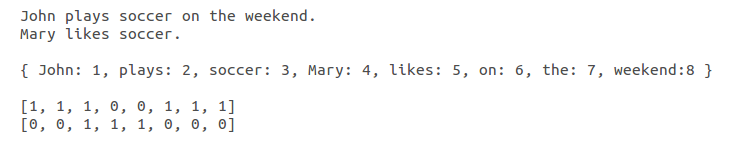
\includegraphics[width=0.8\textwidth]{images/bow}
\caption{A bag of words placed into a vector\label{fig:bow}}
\end{figure*}

Some times to notes about this example. The dictionary constructed in the second step does not have to appear in the same order
that the words are found in the text. After extraction, each word is represented by a 8-entry vector. The terms in the vector
are then subject to weighting. The weighting is preformed by the gradient descent algorithm that was described above and the
weights in the large b-weight vector as previously described. This way of data mining free text fields is very common among
data mining applications.\\

For the actual data mining process, 6 main data trials were given as input to the VW program. These trials and their data varied as
follows. First, a simplistic approach was taken by excluding all bag of words columns in the training instances. Bag of words form
the most complex data mining rules and therefore are excluded to create a base line analysis of where the tool will finish without
any of the added complexity. This data set trial was used with both the logarithmic first and square root functions of data normalization.
(All data trials from now on are used once with logarithmic and once with square root normalization.) These results of these base line
trials runs can be found in Table~\ref{tab:results} in the last section of the paper. The next trial to be run on the data mining algorithm (gradient
descent) was what we call the full bag of words run. Here, all columns that are bag of words and not categorical were used in addition
to all categorical columns. The main note here is that the bag of words columns were pre-processed in order to eliminate numbers, 
abbreviations, or any other text that cannot be classified in a standard dictionary. This pre-processing only leaves English words
in the free text columns of the training instances. The results of this trial run can again be found in Table~\ref{tab:results}. The 
final, and most complex trial run against the gradient descent algorithm was what we are calling bag of keywords. As the title of
this trial gives away, we were only concerned with keywords in the free text columns of the training instances. In order to
get the keywords of a particular bag of text, the python library known as Topia\footnote{https://pypi.python.org/pypi/topia.termextract/}
was used. Topia is a natural language processor library which can (with some flexibility) extract the keywords from a block of text.
An example of keywords are as follows. The text "The fox can't jump over the fox's tail." in Topia yields the results:
[('tail', 1, 1), ('fox', 2, 1)]. As it can easily be seen, the keywords of tail and fox have been extracted from the main body of
text as keywords. What is less obviously are the remaining digits provided by Topia. This is where the flexibility of Topia comes into
play. In each triple, the keyword, the occurrences, and the number of words in the keyword are given. This being the case, we are
able to set thresholds on Topia's extractions in order to limit the keywords selected. We can limit the keywords to only those
repeated in the text body at least once, or those that are composed of at least two words and so on. However, for simplicity of
our main data trials, we allowed Topia the lowest of thresholds for keyword extraction, being no repeat and single words. This
allowed us to again create a base line measurement of keyword usage in the data mining process. Again pre-processing was done on
the training instances in order to limit the free text columns to key words only. The results of this baseline keyword run
in VW can be seen in Table~\ref{tab:results}.\\

Aside from the 6 main trials, 2 additional trials (with square root and log) were given as the global keyword system described in the Data Preparation
section of this paper. This was the final ditch effort used in data mining for this project. Once the global keywords had
been collected by the python script, the CSV to VW script was slightly modified in order to only include the words in the full
description of the job which appeared in the global keyword list. For simplicity, the global keywords list was limited to
500 words as we felt that these keywords are should yield better results compared to a larger list.